\documentclass[a4paper,12pt]{jarticle}
\usepackage[dvipdfmx]{graphicx}
\usepackage{mymacros}
\usepackage{okumacro}
\textheight 9.0in
\textwidth 6.0in
\topmargin 0in
\oddsidemargin .2in
\evensidemargin .2in
\title{
{\LARGE\sffamily\gtfamily
OJL報告書
}
\vspace*{.6in}
{\huge\sffamily\gtfamily
トレースログ可視化ツール TraceLogVisualizer(TLV) に対する機能追加とリファクタリング
}
\vfill\vfill\vfill
}
\author{
\LARGE\sffamily\gtfamily
350702101\ \ \ \ 後藤 隼弐\\
}
\date{
\vfill
\Large\sffamily\gtfamily
名古屋大学 大学院情報科学研究科\\[.2in]
情報システム学専攻\\[.2in]
2010年1月
\vfill
}\renewcommand{\baselinestretch}{1}
\begin{document}

\newcounter{mysection}
\def\thesection{\large\arabic{section}}
\newcommand{\mysection}[1]{\vspace{-2zh}\section{\large #1}\vspace{-0.5zh}}

\newcommand{\step}[1]{\textbf{#1} }

\pagestyle{empty}
%%%%%%%%%%%%%%%%%%%%%%%%%%%%%%%%%%%%%%%%%%%%%%%%%%%%%%%%%%%%%%%%%%%%%%%%%%
% 和文要旨
%-------------------------------------------------------------------------
\vspace*{-1in}
\begin{center}
\large\sffamily\gtfamily トレースログ可視化ツール TraceLogVisualizer(TLV) に対する\\
機能追加とリファクタリング
\end{center}
\begin{flushright}
\large\sffamily\gtfamily
350802246\ \ \ \ 水野 洋樹
\end{flushright}
\begin{center}
\large\sffamily\gtfamily 要旨
\end{center}
{
\setlength{\baselineskip}{0.9\normalbaselineskip}

近年、組込みシステムの分野においてもマルチコアの導入が進んでいる.
マルチコア環境では、各コアが独立し
て並列に動作するため、ブレークポイントやステップ実行を用いた実行時のデ
バッグが困難である.そのため、 RTOS等のトレースログを用いた
デバッグが有用と考えられるが、サイズの大きなトレースログを直接開
発者が扱うのは困難である。そこ
で本OJLでは、トレースログを可視化表示することで解析を容易にし、マルチコ
ア環境でのアプリケーション開発を支援である
\textbf{TraceLogVisualizer(TLV)}の開発を目的とする。

TLVは,各種RTOSやシミュレータ,エミュレータなどが出力するトレースログを
可視化表示するツールである. TLVは,トレースログを変換ルールに従い標準形式トレースログに変換し,
標準形式トレースログに対して可視化ルールを適用し、図形データの生成を行う.
TLVでは,変換ルールと可視化ルールを外部ファイルとして与えることで,汎用
性と拡張性を実現する.

本OJLは図\ref{schedule}のようにフェーズに分割して開発を行なった.
フェーズの終了ごとにTLVのリリースを行ない、要求の収集を行なった。

%% 2008
%% 年度後期のフェーズ3では単体テスト・システムテストと,機能拡張のための要
%% 件抽出を行った.2009年度前期のフェーズ4では要求の収集を行い、スクリプト
%% 拡張機能を実装した。2009年度後期のフェーズ5ではアプリケーションの動作速
%% 度向上を目的として、リファクタリングを行なった。また、フェーズ4の内容を
%% 反映させたバージョン1.1を公開した。

\begin{figure}[b]
\centering
\vspace{1zh}
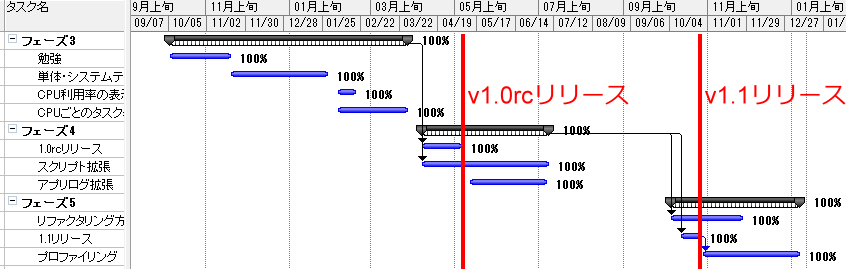
\includegraphics[width=0.9\textwidth]{whole_schedule.png}
\caption{全体スケジュール}\label{schedule}
\end{figure}

リリースを通じて要求を収集したところ、(1)従来の変換ルール,可視化ルールでは行なえない
複雑な可視化を行いたい、(2)トレースログの解析が遅いため高速化して欲しい、という要求が強かった。

(1)の複雑な可視化を実現するために、
\MARU{1}変換ルールと可視化ルールを拡張する
\MARU{2}変換用の言語を開発する
\MARU{3}外部プロセスで変換・図形生成を行なえるようにする、
の3つの方針を比較検討した。
実装コストを利用者の学習コストを考慮し、\MARU{3}の方法を選択し、
変換と図形生成を外部のプロセスで行なえるよう
にするスクリプト拡張機能を実装した。外部プロセスは任意のプログラミング
言語で記述できるため、複雑な可視化を行なえる。

%(1)変換ルールと可視化ルールを拡張する
%(2)変換用の言語を開発する
%(3)外部プロセスで変換・図形生成を行なえるようにする、
%の3つの方針を比較検討した。

%% (1)の方法はルールが複雑化しているため実装コストが大きい。
%% (2)の方法も新たな言語の設計が必要であるため実装コストが大きい。
%% また利用者が新たな言語を学習する必要がある。
%% そこで、実装コストを利用者の学習コストを考慮し、(3)の方法を選択した。

%% スクリプト拡張を行なった後のTLVの変換プロセスを図\ref{fig:se}に示す。外
%% 部プロセスは任意のプログラミング言語で記述できるため、複雑な可視化を行
%% なえる。外部プロセスとは、標準入出力によって通信が行なわれる。

%% スクリプト拡張によって、CPU利用率の可視化を行なった例を図\ref{fig:cpu}に示す。

%% \begin{figure}[b]
%% \begin{minipage}{0.45\columnwidth}
%% \centering
%% \includegraphics[width=\textwidth]{se.eps}
%% \caption{外部プロセスによる変換・図形データの生成の実現}\label{fig:se}
%% \end{minipage}
%% \begin{minipage}{0.45\columnwidth}
%% \centering
%% 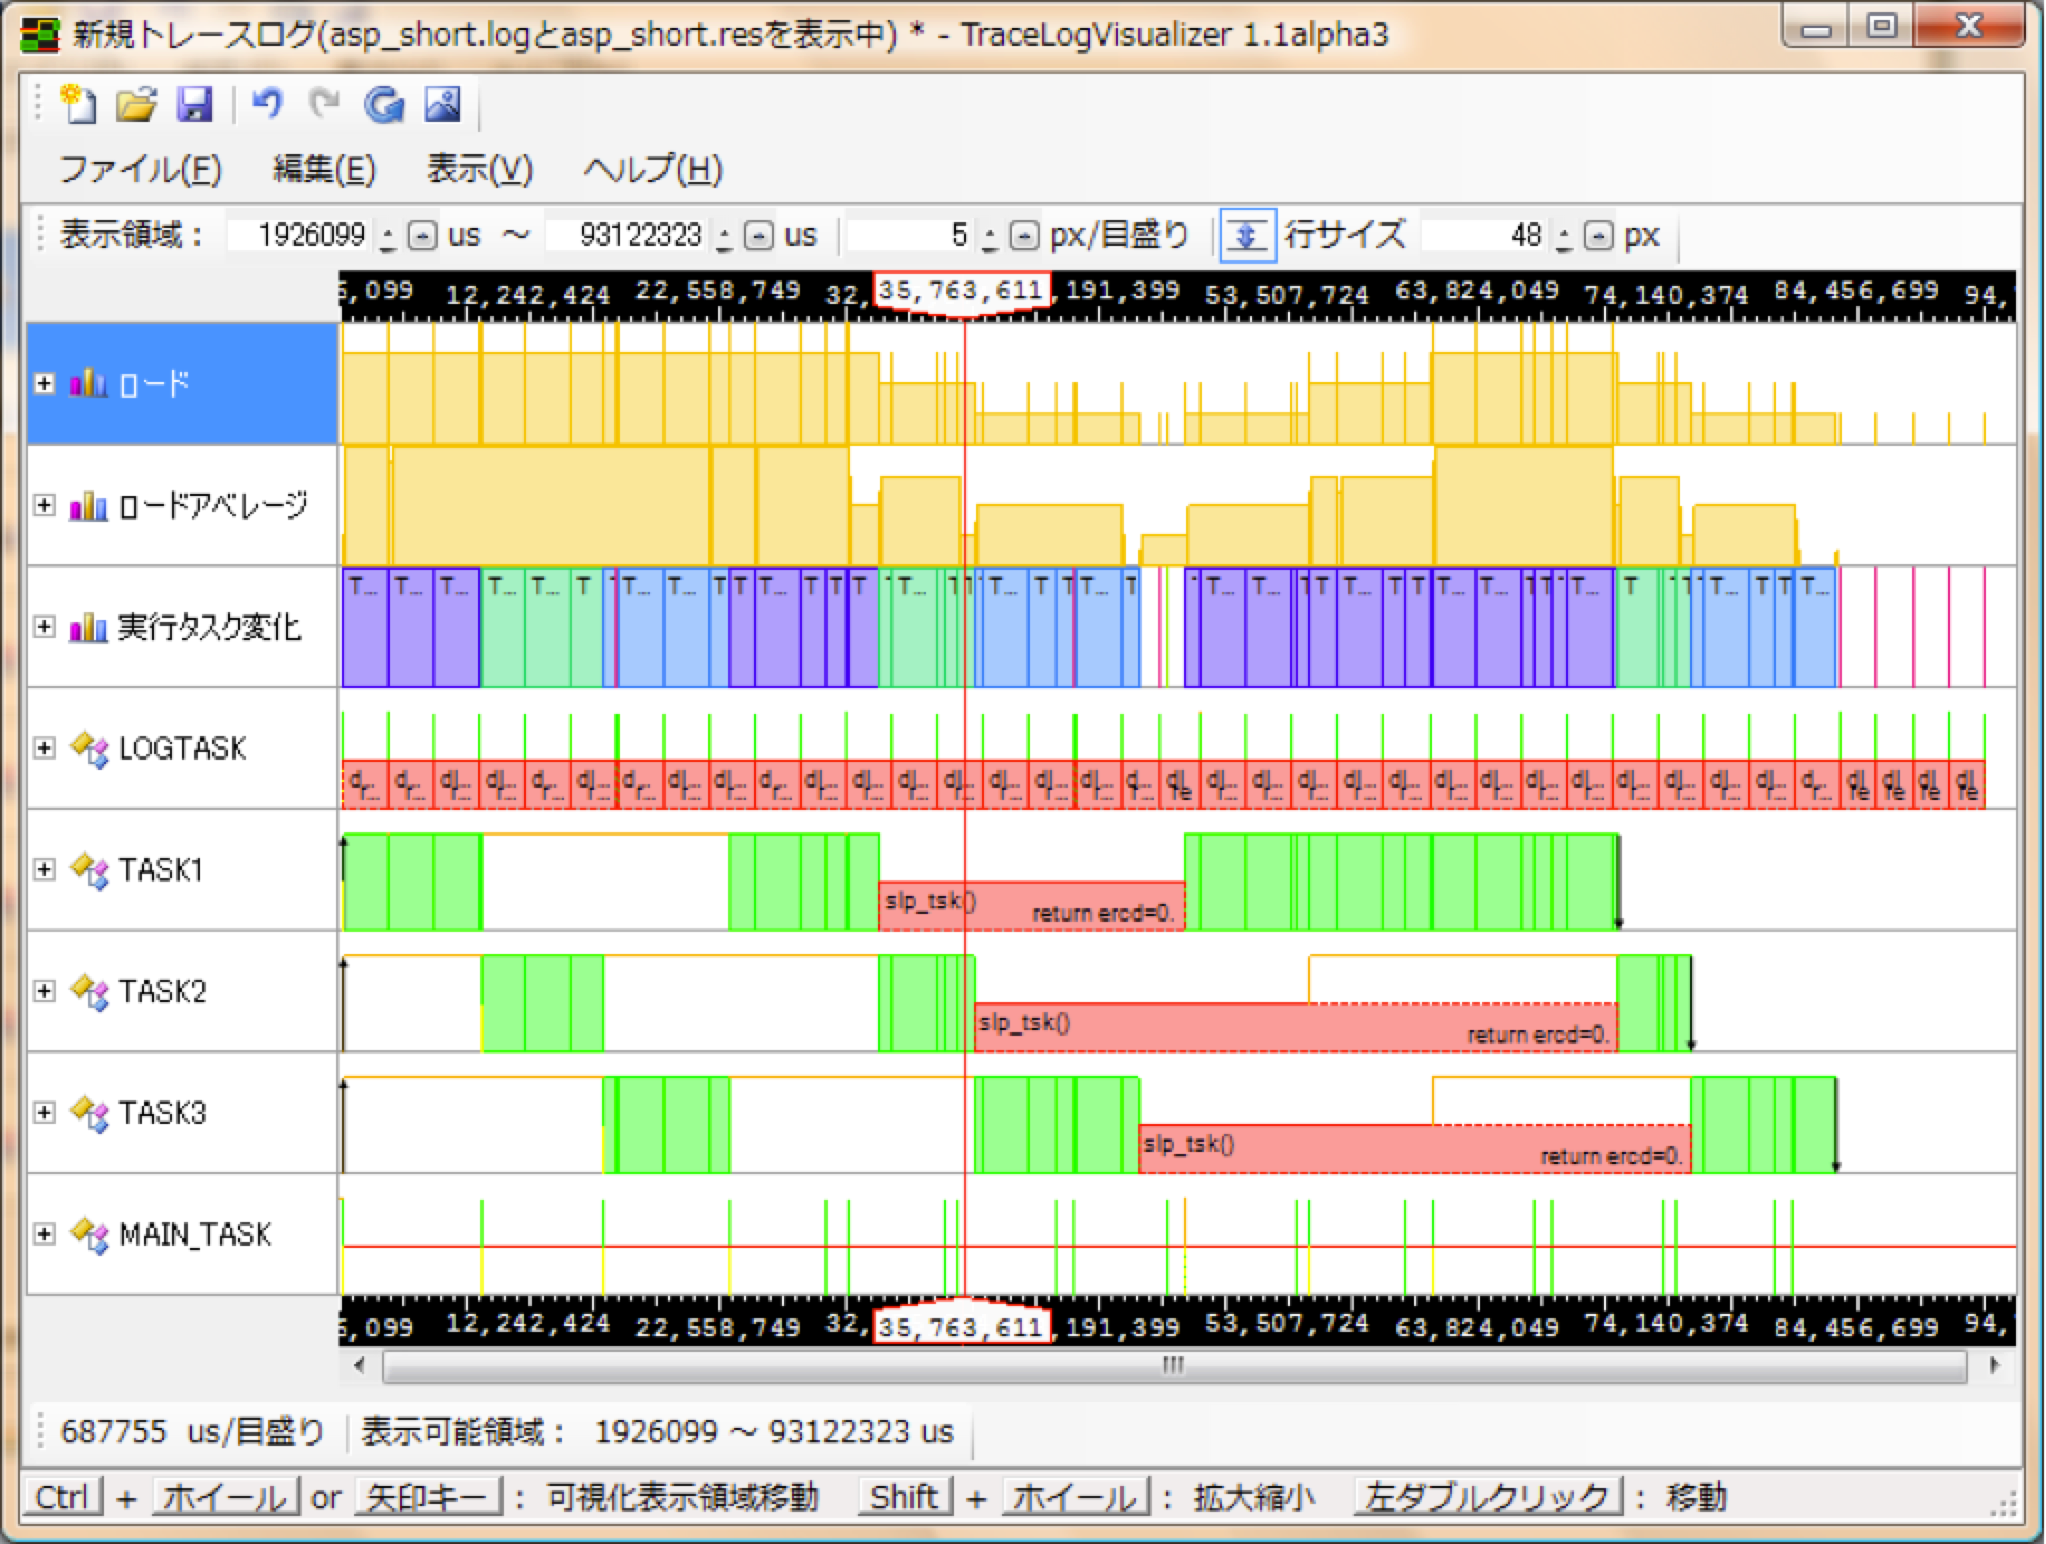
\includegraphics[width=0.8\textwidth]{cpu.png}
%% \caption{CPU利用率の可視化}\label{fig:cpu}
%% \end{minipage}
%% \end{figure}

(2)の変換の高速化の行なうにあたり、トレースログへの変換に関するソースコー
ドが複雑化している点が障害となった。そこで,関連するソースコードの調査
した。
調査の結果、クラス設計に大きな問題はなかったが、
多くのクラスにおいて、複雑な処理を行なうメソッドが存在しており、これが
ソースコードを複雑化さている原因であった。
そこで、複雑化したメソッドの整理をリファクタリングの目的とした。

%% クラスを調査した結果、多くのクラスにおいて,複雑な処理を行なうメソッドが存在しており,こ
%% れがソースコードを複雑化さている.そこで,メソッドの整理する
%% ための共通機能のくくりだしやクラス分割をリファクタリングの目的とした.

%% 標準形式トレースログの解析が,複雑な正規表現が多用により複雑化していた。
%% これを改善するためは,正規表現ではなく文脈
%% 自由文法を扱えるパーサを採用する必要がある.パーサの実現方法について,
%% (1)Yaccなどのコンパイラ・コンパイラの利用
%% (2)Parsecなどのパーサコンビネートの利用、
%% の2つの方針を検討した。
%% パーサを再生成する必要がない点やデバッグの容易さなどから,2 つめのパー
%% サ・コンビネータを用いる方針を採用した.

%% 可視化ルールは木構造を持つが、
%% そのクラスは木構造ではない。
%% 木構造をトラバースする処理がさまざまな場所で重複して記
%% 述され,保守性を低下させている.これを改善するために,Figuresクラスに
%% Compositeパターンを適用し,明示的に木構造を表現する.また,
%% 処理の拡張を容易にするためにVisitorパターンを適用する.

%% 複数のFiguresクラスの集約によって表
%% 現される.FiguresクラスにはShapeとFigures の二種類が存在し,Figuresは複
%% 数のShapeによって構成されという木構造をもつ.しかし,木構造として表現さ
%% れていないため,木構造をトラバースする処理がさまざまな場所で重複して記
%% 述され,保守性を低下させている.これを改善するために,Figuresクラスに
%% Compositeパターンを適用し,明示的に木構造を表現する.また,Figures
%% をトラバースする処理の拡張を容易にするためにVisitorパターンを適用する.
}

\end{document}
